\chapter{Implementation}
\label{chap:implementation}

To feed the batch optimization, data needs to be collected.
Data from simulation and from a real blimp are used in this work.
The content of a dataset and its implementation in \textsc{Matlab} are explained first in this chapter.
Then, the methods used to generate these datasets from a real blimp and from simulation are shown.

\section{Dataset}
\label{sec:dataset}
The \textsc{Matlab} implementation of the batch optimization takes a dataset as the input and returns a set of optimal parameters estimated from the given dataset. \\
A dataset is designed to be self contained. 
Each dataset includes information about the structure of the system and a set of input vectors with their corresponding measurement vectors from the sensors. \\
In the current implementation the structure contains the true values\footnote{
True values are only known for the simulation datasets. 
For datasets from the real blimp, the true values are not known and therefore replaced with values based on the CAD files of the blimp.}
for the motor positions and their coordinate system transformations, the blimp radius, the blimp mass and the inertia tensor as well as transformation matrices for the sensors. \\
The measurement data is stored in segments.
A segment is a homogeneous sequence of continuously sampled actuator feedback vectors as well as measurement vectors.
Because the real system exhibits transients upon changing inputs a boolean is also stored for each data-point which denotes whether the system has reached steady-state. \\
With this technique it is possible to easily cut away parts of segments which have disturbances in them while still preserving transient information.

\section{Real System}
\label{sec:real_system}
To record data from a real blimp, experiments where conducted on the Skye System. \\
To excite the system with actuator inputs which are suitable for batch optimization, we expanded both \textsc{QGroundControl} and the Skye specific PX4 firmware with new functionality.

\subsection{Input Patterns}
\label{sub:input_pattern}
We tried a number of different approaches to input patterns.
There are two main goals for the design of the input pattern:
\begin{enumerate}
\item The input must be \textbf{persistent of excitation}. Basically, that means that thrust magnitude and direction of the input forces must be uncorrelated.
\item The input must be \textbf{applicable}. Because there are obstacles in the surroundings of the blimp (ground, hangar walls, etc.), the movements should be as small as possible.
\end{enumerate}

Another aspect of the real system is that it takes some time until the actuators have reached the desired orientation and thrust.
Those transients are very hard to estimate, mainly because the thrust motor controller has no feedback and exhibits very high variability in its dynamic behaviour.
In addition to the unknown thruster dynamics, the hull also reacts to load changes with vibrations that influence the IMU measurements. \\

By combining these constraints on the inputs, we came up with the following pattern scheme:
\begin{enumerate}[(i)]
\item Apply input vector to system for a fixed amount of time
\item Stop thrust and turn actuators in the opposite direction
\item Apply same input vectors in reverse for the same amount of time
\end{enumerate}
Using this scheme, the velocity of the system yields nearly zero after the pattern when starting with zero velocity\footnote{To reach not only zero velocity but also zero position shift after the pattern, a \textit{forward-backward-backward-forward} pattern would be possible. However, this pattern needs double the time for execution and since only feed-forward control is applied, the position drift is not much smaller than for the shorter pattern.
}.
This enables to sequently apply multiple of those patterns before the system must be repositioned.
\\

For the input vectors themselves, pseudo random sequences would be most promising.
However, the elaboration of the optimal input sequences goes beyond the context of this work and we tested the following options:
\begin{enumerate}[(a)]
\item Generate normally distributed angular acceleration vectors and use allocation to generate input vectors for the thrusters (this leads to angular acceleration only and no translations)
\item Use fixed thrust and select thruster angles from a uniform random number distribution
\item Generate normally distributed thrust vectors and select thruster angles from a uniform random number distribution
\end{enumerate}
It figured out, that (a) is not persistent in excitation.
This actually becomes clear when having a look at $\mathbf{M}^{actuation}$ from \cref{eq:moments}.

\begin{equation}
\label{eq:m_actuation}
\mathbf{M}^{actuation} = \sum_{k=1}^N  \left[  \mathbf{C}_{b,m_k} \left( \mathbf{p}^{m_k,cog}_{m_k} \times \mathbf{F}^k_{m_k} \right)  \right]
\end{equation}

The allocation is basically the inversion of $\mathbf{C}_{b,m_k} ( \mathbf{p}^{m_k,cog}_{m_k})^\times$, i.e. a mapping $\mathbb{R}^{2N} \rightarrow \mathbb{R}^3$.
If the allocation is used to feed $\mathbf{F}^k_{m_k}$, only a subspace of the domain of $\mathbf{F}^k_{m_k}$ is used and the problem yields unobservable.
\\

From the remaining options (b) and (c), it turns out that the variant with random thrust magnitude is better than the other one, because method (b) still only excites a sub-space of the input space.
This is prevented using fully random inputs provided by method (c).

\subsection{Input Generation}
\label{sub:input_generation}
To avoid having to re-flash the firmware all the time, the inputs are generated inside \textsc{QGroundControl} and directly forwarded to the actuators via the controller of the blimp.
This way, all of the parameters like standard deviation and time intervals can be set from within the \textsc{QGroundControl} interface.

\begin{figure}[H]
\centering
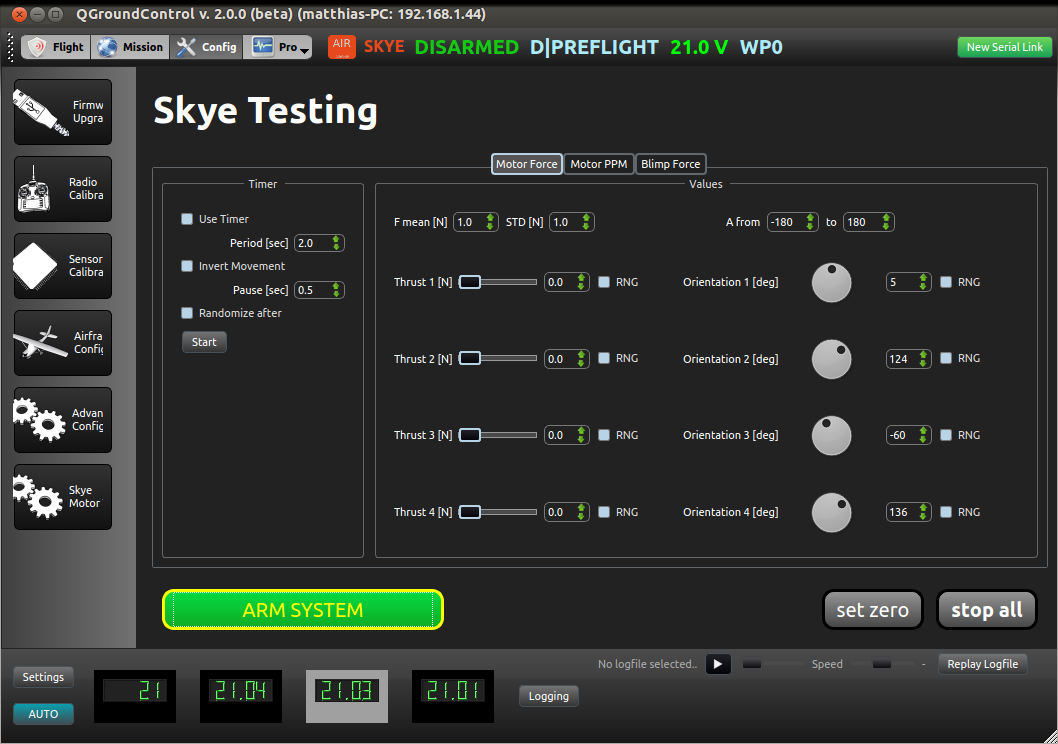
\includegraphics[width=.9\textwidth]{images/qgc/QGroundControl_v_2.png}
\caption{\textsc{QGroundControl} input generation interface. Time intervals and random number specifications can easily be changed. The transmission of the input sequence can be started and stopped.}
\label{fig:qgc_input_gen}
\end{figure}

\begin{figure}[H]
\centering
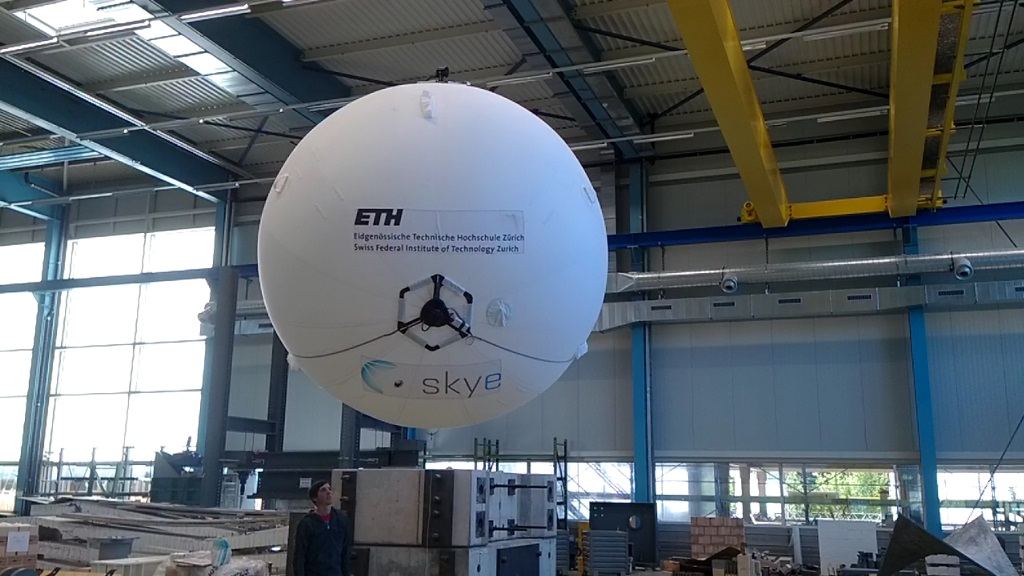
\includegraphics[width=.9\textwidth]{images/foto_testing_setup.jpg}
\caption{Test setup for data generation. One operator initiates the input pattern at the ground station (not visible), the second operator repositions the blimp when it approaches too close to an obstacle after some input sequence.}
\label{fig:test_setup}
\end{figure}

\subsection{Test Setup}
\label{sub:testing_setup}
Although the input patterns are designed to avoid large movements as good as possible, the blimp still needs to be catched after a number of such inputs.
This leads us to the basic testing setup we used to record data: \\

An operator is located at the ground station and a second operator is near the blimp.
At the ground station there is a button to initiate one such input pattern.
The second operator at the blimp catches it as soon as it drifts too close to an obstacle (see \cref{fig:test_setup}). \\
With this setup it was possible to initiate an input patterns roughly every 6 seconds. 
This is including the time needed to reposition the blimp when it has drifted too much.



\subsection{Data Acquisition}
\label{sub:data_acquisition}
For accurate feedback from the blimp the firmware was extended to offer a mode where it will transmit the relevant sensor and actuator feedback data to the ground station. \\
The new mode collects and transmits the following data to the ground station:
\begin{enumerate}
\item raw gyro
\item raw accelerometer
\item angular acceleration from EKF
\item angular rate from EKF
\item orientation quaternion from EKF
\item thrust of each actuator (from thrust signal that is passed to the thrust motor controller)
\item orientation angle of each actuator (from motor encoder)
\end{enumerate}
The actuator feedback loop runs at \unit[25]{Hz}.
Hence the whole telemetry message is transmitted at that rate.
To avoid problems with noise aliasing the sensor signals are run through a resampling filter.\\
\textsc{QGroundControl} then writes these mavlink messages into a log-file that serves as an input for generating a dataset for the optimization with \textsc{Matlab}.

\subsection{Data Selection}
\label{sub:data_selection}
After a raw dataset has been recorded it needs to be preprocessed to be usable for our batch optimization code.
\Cref{fig:data_selection_long} shows a period of multiple segments of the dataset and \cref{fig:data_selection_short} shows one segment in more detail.
\\

First after importing a raw dataset, the regions where thrust transients are to be expected are marked in the dataset.
This process is implemented with generous margins to eliminate problems with the batch optimization.

\begin{figure}[htbp]
\centering
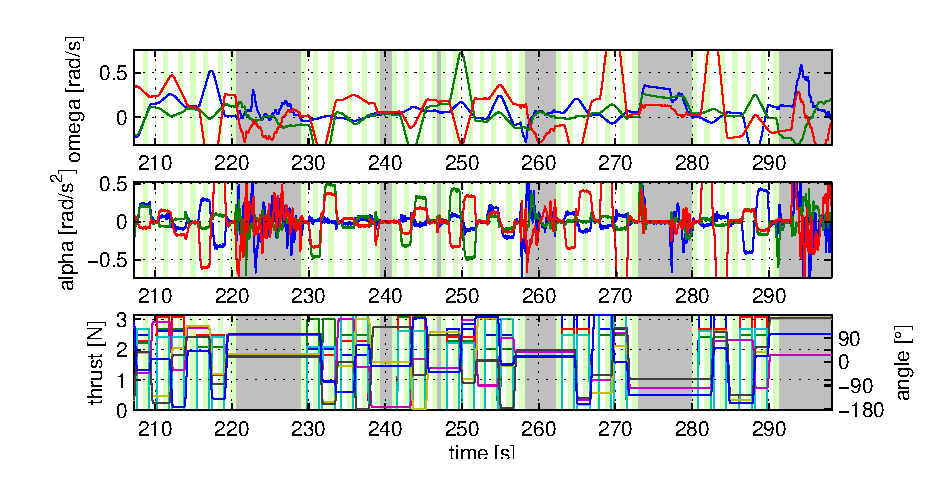
\includegraphics[scale=0.8]{images/interactive_cut/interactive_cut_long_modified.eps}
\caption{Except of dataset after transient marking. \textbf{Gray} regions are the values out interest (no inputs for a time longer than a threshold). \textbf{White} regions are the thrust transient parts which are discarded. \textbf{Green} regions are the remaining data which is used for batch optimization.}
\label{fig:data_selection_long}
\end{figure}

Then the segments where the blimp has been catched and repositioned need to be cut from the dataset. \\
For this purpose a semi-automatic cutting tool was implemented (see \cref{fig:data_selection_short}). 
The tool first identifies the segments of interest and then displays each of them to the use for visual inspection.
The user can then adjust the borders of the segments to cut away any visible disturbances. \\
Good and bad segments are easily distinguished by looking at the angular acceleration plot.
An undisturbed system shows constant angular accelerations during the periods where the thrusters are active. \\
Using this approach to select datapoints within a dataset, only about 50\% of the raw data from the session has to be discarded.
The result is a dataset with undisturbed system response including transients.
When the described transient removal is applied, about 40\% of transient-free data remains.\\
To summarize: for 10 seconds of transient-free data about 50 seconds of raw data has to be collected.

\begin{figure}[htbp]
\centering
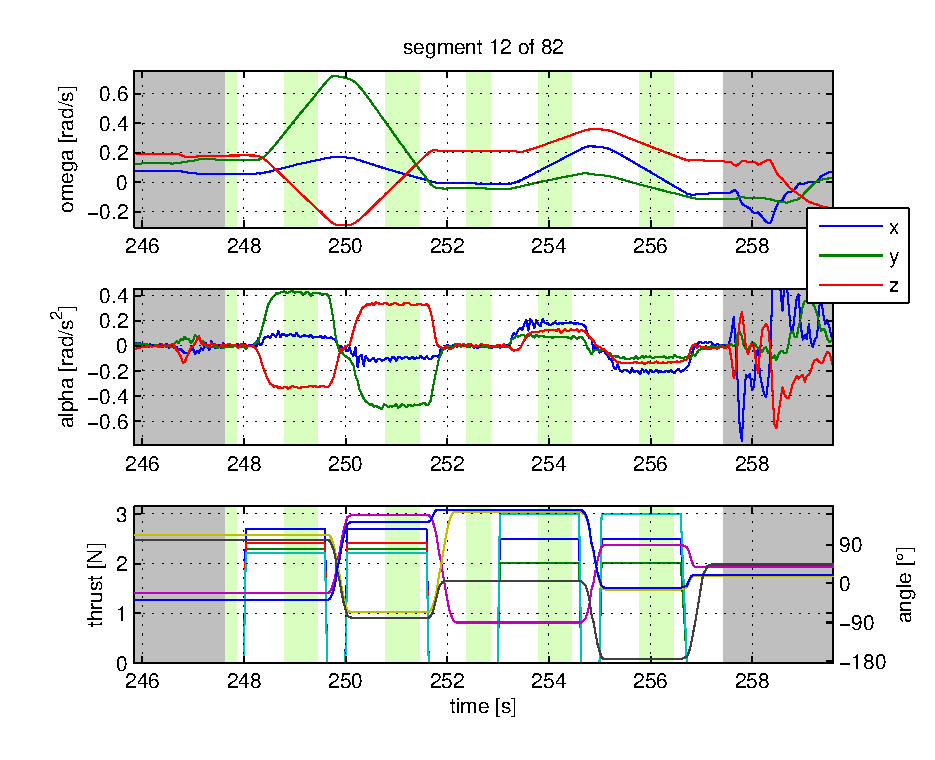
\includegraphics[scale=0.8]{images/interactive_cut/interactive_cut_detail_modified.eps}
\caption{Cutting tool displaying one segment of the dataset. 
The \textbf{green} regions which are used for the batch optimization do only contain data with steady-state thrust. 
The \textbf{white} thrust transient regions are defined with a generous margin.
As there is no feedback about the thrust motor, this data is discarded.
Vibrations of the hull caused by load changes are also visible in these regions.
Disturbances can be clearly seen in the \textbf{grey} regions.
}
\label{fig:data_selection_short}
\end{figure}

\section{Simulation}
\label{sec:simulation}
A blimp simulator was implemented for several reasons:
\begin{itemize}
\item fast turn around time for generating new datasets
\item disturbance (like sensor noise or aerodynamic drag) can be turned on and off
\item different blimp configurations can be evaluated without having a new prototype
\end{itemize}

Combining those reasons with the properties of the data selection procedure (see \cref{sub:data_selection}), the following requirements were considered for the simulation:
\begin{itemize}
\item include aerodynamic drag
\item include sensor noise
\item include thruster dynamics
\item allow for easy reconfiguration of the blimp
\end{itemize}
The simulation was implemented as object oriented \textsc{Matlab} code.
\Cref{fig:sim_tree} gives an overview about the code architecture.
% XXXXXXXXX add reference to UML diagram in appendix here

The blimp is built with objects that interact with each other.
Each of these objects can have continuous and discrete states.
The simulator then interacts with the objects over a standardized interface.
At each time-step the simulator updates the states of the objects and then calls a function on each object to calculate the derivatives of the continuous states.
Additionally, at the border of a discrete time step the simulator also calls a function on the objects to get the next discrete states.

\begin{figure}[htbp]
\centering
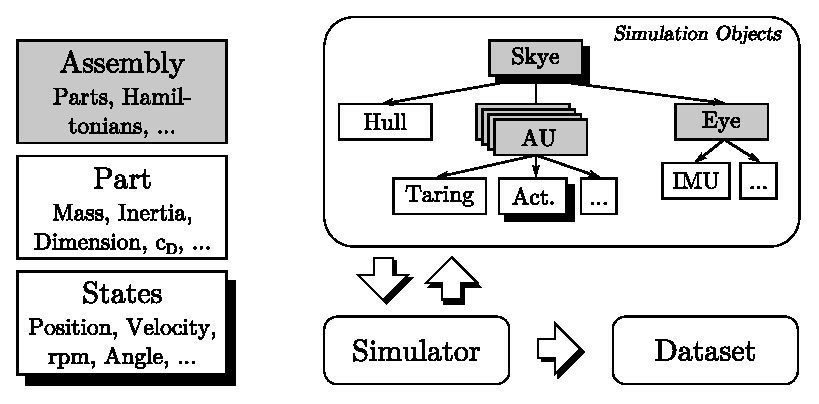
\includegraphics[width=0.9\textwidth]{images/sim/sim_tree.eps}
\caption{Tree like data-structure of simulation objects. Assembly parts (\textbf{gray}) have subparts (\textbf{white}) and hold additional information about their arrangement. Some parts include states (\textbf{shaded}). The simulator interacts with the simulation objects and generates a dataset.}
\label{fig:sim_tree}
\end{figure}

\subsection{Motion Equation}
\label{sub:motion_equation}
At the core of the blimp simulation is a the rigid body dynamics model. 
The simulator uses the same motion equation as described in \cref{tab:sys_mod}.

\subsection{Mechanical Properties}
\label{sub:mech_properties}
To calculate the mechanical properties, the blimp structure is represented in a tree like data-structure (see \cref{fig:sim_tree}).
The root node of the tree is the actual rigid body object which is simulated by the simulator.
Each node in the tree represents an assembly of parts. \\

With this methodology the blimp is actually an assembly of several parts. 
In general it will include a hull, the electronics unit and a number of actuation units.
Each of these parts are assemblies by themselves.
The electronics unit could include for example the cover, a camera and the PX4FMU, which simulates the sensors.\\
An actuation unit is also an assembly of for instance a battery, a taring weight and an actuator which simulates the actuator dynamics and generates the forces.\\
This concept allows to have different types of components in a library which can then be used to build an arbitrary blimp. \\

After the blimp has been assembled, the mechanical properties of the parts at the leafs of the tree data-structure are recursively combined into their parent node.
This way the mechanical properties of the root node are recalculated.\\
The taring routine uses the tree structure to calculate values for the taring weights located at the actuation units. 
After taring is done, the changed mass of the taring weights cause the tree to recalculate the mechanical properties of the root node.

\subsection{Aerodynamic Drag}
\label{sub:aero_drag}
The aerodynamic effects are the most difficult part of modelling.
Aerodynamic drag is usually separated into \textit{form drag}, \textit{wall friction drag}, \textit{interference drag}, \textit{lift-induced drag} and \textit{wave drag} which are listed in decreasing importance for blimp modelling\footnote{
Wave drag describes compression effects of the fluid and is not relevant for subsonic speed.
Lift-induced drag is also neglected because blimps we consider blimps as symmetric profiles without considerable angle of attack.
Interference drag is assumed low, as the actuation units and other components on the blimp are much smaller than the hull and is therefore also neglected.
}.\\

We modelled \textit{form drag} for translational movements and \textit{friction drag} for rotational movements as quadratic functions w.r.t. to the velocity.
Further, a \textit{virtual mass factor} was considered for the hull to consider the inertia of the surrounding fluid.
\textit{Form drag} was applied to the hull and the actuation units which are represented by cylinders with appropriate dimension.
\textit{Friction drag} was applied to the hull for rotational speed only.
Together with the form drag of the actuation units, the friction drag of the hull acts as a damping moment on rotational movements.\\

Form drag coefficients\footnote{
Blimps like Skye are close to the drag crisis point of spheres ($Re\approx3e05$). Interpolation of the drag coefficient according to the actual velocity is used.}
and virtual mass factor were introduced according to the literature \citep{Kundu2012}.
The friction drag coefficient of the hull was determined such that the rotational resistance coincides with reference measurements.

\subsection{Thruster Dynamics}
\label{sub:thrust_dynamics}
The actuator has been modelled according to test-bench measurements\footnote{The use of test-bench measurements are by courtesy of Daniel Meier.} of the thruster.
The dynamic thruster model includes:
\begin{itemize}
\item thrust start-up delay
\item thrust reaction delay
\item minimum and start-up thrust thresholds
\item second order thrust motor dynamics
\item rotation actuator maximum speed
\item second order rotation actuator dynamics
\end{itemize}
The thruster dynamics has been implemented as a blackbox model.
The minimal parameters needed to describe the listed properties of the thruster dynamics are matched to the test-bench measurements using an empirical approach.  \\
Because the thruster dynamics are not critical to our application this yields sufficient accuracy.

\subsection{Inertial Sensors Model}
\label{sub:imu_model}
Following the idea of the simulator framework the inertial sensors are also an object which is attached to the blimp assembly. \\
The tree-like framework of the simulation objects is bidirectional.
While the mechanical properties of the leaves are used to determine the properties of the root,
the motion of the rigid body at the root of the structure is distributed to each of the leaf nodes in their respective coordinate systems. \\
The sensor object then only has to take the already transformed accelerations, velocities and orientations and store them.
In this process the sensor object also adds noise to the sensor values.

